\documentclass[../main]{subfiles}

\questiontrue
\solutiontrue

\begin{document}
    \ifquestion
    
	
    \section{Variable Solar "Constant"}
	
	Safira's house is a cube with 5 windows: one on each vertical wall and one on the roof, each with a cross-sectional area $A$. Observing the house from above, one notes that the angle of inclination of the house's axis with the projection of the local meridian is $\theta$, as shown in Figure \ref{fig:safira}.
	
    \begin{figure}[htpb]
	    \centering
	    

\tikzset{every picture/.style={line width=0.75pt}} %set default line width to 0.75pt        

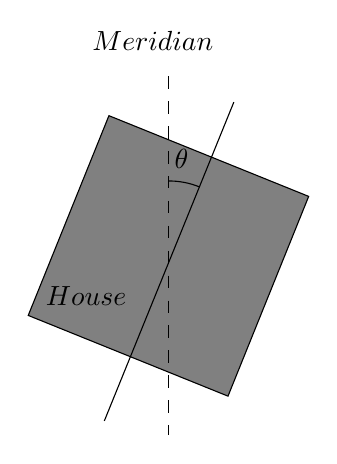
\begin{tikzpicture}[x=0.75pt,y=0.75pt,yscale=-1,xscale=1]
%uncomment if require: \path (0,408); %set diagram left start at 0, and has height of 408

%Shape: Square [id:dp23931407551563044] 
\draw  [fill={rgb, 255:red, 128; green, 128; blue, 128 }  ,fill opacity=1 ] (284.42,156.01) -- (380.66,194.9) -- (341.78,291.14) -- (245.54,252.25) -- cycle ;
%Straight Lines [id:da6822891895825496] 
\draw  [dash pattern={on 4.5pt off 4.5pt}]  (313.1,137.09) -- (313.1,310.06) ;
%Straight Lines [id:da5128085036827124] 
\draw    (344.6,149.48) -- (282.2,303.07) ;
%Shape: Arc [id:dp3372338716191585] 
\draw  [draw opacity=0] (312.95,187.48) .. controls (313.1,187.48) and (313.25,187.47) .. (313.4,187.47) .. controls (318.49,187.47) and (323.36,188.46) .. (327.81,190.24) -- (313.4,226.27) -- cycle ; \draw   (312.95,187.48) .. controls (313.1,187.48) and (313.25,187.47) .. (313.4,187.47) .. controls (318.49,187.47) and (323.36,188.46) .. (327.81,190.24) ;  

% Text Node
\draw (314.85,171.08) node [anchor=north west][inner sep=0.75pt]    {$\theta $};
% Text Node
\draw (275.2,113.88) node [anchor=north west][inner sep=0.75pt]    {$Meridian$};
% Text Node
\draw (252.8,236.88) node [anchor=north west][inner sep=0.75pt]    {$House$};


\end{tikzpicture}
	
\caption{Geometric positioning of Safira's house}
\label{fig:safira}
\end{figure}

\ut{a} Find the Sun's altazimuthal coordinates as a function of its declination $\delta$, the time elapsed since true solar noon $t$ ($t<0$ for before noon), and the local latitude $\phi$.

\ut{b} Find an expression for the radiation luminosity entering the house as a function of the previous parameters, the window area, and the solar constant.

\ut{c} Sapphire, upset with her excessive energy costs, decided to install a solar panel system to collect energy. However, she did not plan properly and ended up installing the panels inside her house, and also renovated her house and covered all the side windows. Thus, find the total energy obtained by the panel over a full day.

\textbf{Data:}
\begin{itemize}
    \item Total area of the panels: $A_p$
    \item Side length of the house: $L$
    \item Window area: $A_j$
    \item The top window has a film that allows radiation to enter but not escape. Also consider that the walls are reflective and the brightness becomes homogeneous inside the house.
\end{itemize}

\clearpage
\fi
\ifsolution


\section{Variable Solar "Constant"}

\ut{a} Using the well-known relationships of altazimuthal coordinates:

$$\cos(H) = \frac{\sin(h) - \sin(\delta)\sin(\phi)}{\cos(\delta)\cos(\phi)}$$

Such that:

$$\sin(h) = \cos(H)\cos(\phi)\cos(\delta) + \sin(\phi)\sin(\delta)$$

And from spherical triangle relations, we can show that:

$$\frac{\cos(h)}{\sin(H)} = -\frac{\cos(\delta)}{\sin(A)}}$$

Therefore:

$$\sin(A) = -\frac{\sin(H)\cos(\delta)}{\cos(h)}$$

Note that $H = \omega t$, where $\omega = \dfrac{2\pi}{T}$ and $T = 24h$.

From this, we obtain the desired functions:

$$\sin(h) = \cos(\omega t)\cos(\phi)\cos(\delta) + \sin(\phi)\sin(\delta)$$

$$\sin(A) = -\frac{\sin(\omega t)\cos(\delta)}{\sqrt{1 - (\cos(\omega t)\cos(\phi)\cos(\delta) + \sin(\phi)\sin(\delta))^2}}$$

\ut{b} In this case, we need to consider the angle that sunlight makes when entering each window, since it determines how much light actually enters the house. To do this, we project the normal vector of each window onto the celestial sphere (essentially projecting the window itself onto the celestial sphere). These windows have the following projections $(h,A)$:

$$(0, \theta)$$
$$\left(0, \frac{\pi}{2} + \theta \right)$$
$$\left(0, \pi + \theta \right)$$
$$\left(0, \frac{3\pi}{2} + \theta \right)$$
$$\left(\frac{\pi}{2}, 0 \right)$$

The amount of radiation entering a given window is the solar flux (solar constant $F$) multiplied by the area perpendicular to the radiation: $A_t = A \cos(\Delta)$.

The angle $\Delta$ can be calculated using spherical trigonometry:

$$\cos(\Delta) = \sin(h_1)\sin(h_2) + \cos(h_1)\cos(h_2)\cos(A_1 - A_2)$$

For each window we have:

$$\cos(\Delta) = \cos(h)\cos(A - \theta)$$
$$\cos(\Delta) = \cos(h)\sin(A - \theta)$$
$$\cos(\Delta) = -\cos(h)\cos(A - \theta)$$
$$\cos(\Delta) = -\cos(h)\sin(A - \theta)$$
$$\cos(\Delta) = \sin(h)$$

Notice that if $\cos(\Delta) < 0$, the angle is larger than 90º, so the ray will not even enter the window. Therefore, we only consider positive values for the above expressions. Hence, the total luminosity entering through all windows is:

$$L = F A \left( |\cos(h)\cos(A - \theta)| + |\cos(h)\sin(A - \theta)| + |\sin(h)| \right)$$

\ut{c} In the case where all windows are blocked except the top one, the fraction of flux entering the house is $F_\odot \cos(\Delta) = F_\odot \sin(h)$ or:

$$F = F_\odot \left( \cos(\omega t)\cos(\phi)\cos(\delta) + \sin(\phi)\sin(\delta) \right)$$

The power reaching a panel of area $A_p$ is the total power distributed over the area of radiation incidence. After reflections on the walls, the whole room is uniformly illuminated. The total power is $P_t = F A_j$, while the power reaching each wall is $P_i = F \frac{A_j A_p}{6 L^2}$. Since $P = \frac{dE}{dt}$:

$$dE = \frac{A_p A_j}{6 L^2} F_\odot \left( \cos(\omega t)\cos(\phi)\cos(\delta) + \sin(\phi)\sin(\delta) \right) dt$$

Integrating this result, we have:

$$\Delta E = \frac{A_p A_j}{6 L^2} F_\odot \left( \cos(\phi)\cos(\delta)\frac{1}{\omega} \left( \sin(\omega t_f) - \sin(\omega t_i) \right) + \sin(\phi)\sin(\delta) (t_f - t_i) \right)$$

From the solutions of $\sin(h) = 0$, we find:

$$
\begin{cases}
t_i = -|\arccos(-\tan(\phi)\tan(\delta))| \frac{1}{\omega} \\
t_f = |\arccos(-\tan(\phi)\tan(\delta))| \frac{1}{\omega}
\end{cases}
$$

Therefore:

$$\Delta E = \frac{A_p A_j}{3 \omega L^2} F_\odot \left( \sqrt{\cos(\phi - \delta) \cos(\phi + \delta)} + \sin(\phi)\sin(\delta) |\arccos(-\tan(\phi)\tan(\delta))| \right)$$

The value of $\omega$ is given relative to the period of a solar day: $\omega = \frac{2 \pi}{T_\odot}$.

	$$\Delta E = \frac{A_pA_j}{6\pi L^2}F_\odot T_\odot\left(\sqrt{\cos{(\phi-\delta)}\cos{(\phi+\delta)}} +\sin{(\phi)}\sin{(\delta)}|\arccos{(-\tan{(\phi)}\tan{(\delta)})}|\right)$$
	
	
	\clearpage
	
    
    \fi
\end{document}
